\documentclass[main.tex]{subfiles}

\begin{document}

\section{Priority GV}
\usingnamespace{pgv}

This section presents Priority GV (PGV), a session-typed functional language based on GV~\cite{wadler15,lindleymorris15}, but with a twist: it enforces deadlock freedom through priorities \`{a} la Kobayashi~\cite{kobayashi06,padovaninovara15}.

GV enforces deadlock freedom with a syntactic restriction: it fuses channel creation and thread spawning into a single function, called fork. This guarantees that if some term $\tm{L}$ has the means to communicate with both $\tm{M}$ and $\tm{N}$, then $\tm{M}$ and $\tm{N}$ cannot communicate amongst themselves. In other words, GV only allows tree-shaped communication structures, so it is trivially free from cycles, and therefore deadlocks. However, this is overly restrictive, as we rule out \emph{all} cyclic communication structures, not just those with deadlocks.

Priority GV offers a more fine-grained analysis of the communication structure. It allows cyclic communication structures,  and as a result, it is more expressive. To illustrate this, we use PGV to implement an instance of Milner's Cyclic Scheduler in~\todo{Add reference}.

\subsubsection{Types}
Types in PGV are divided into \emph{session types} $\ty{S}$ and \emph{types} $\ty{T}$, $\ty{U}$.
%
Session types are defined by the following grammar:
\[
\begin{array}{lcl}
  \ty{S}
  & \coloneqq & \ty{\tysend[\cs{o}]{T}{S}}
    \sep        \ty{\tyrecv[\cs{o}]{T}{S}}
    \sep        \ty{\tyends[\cs{o}]}
    \sep        \ty{\tyendr[\cs{o}]}
\end{array}
\]
The session types $\ty{\tysend[\cs{o}]{T}{S}}$ and $\ty{\tyrecv[\cs{o}]{T}{S}}$ describe the endpoints of a channel over which we send or receive a value of type $\ty{T}$, and then proceed as $\ty{S}$. The types $\ty{\tyends[\cs{o}]}$ and $\ty{\tyendr[\cs{o}]}$ describe endpoints of a channel whose communication has finished, and over which we must synchronise before closing the channel. Each connective in a session type is annotated with a \emph{priority} $\cs{o}\in\mathbb{N}$.

Types are defined by the following grammar:
\[
\begin{array}{lcl}
  \ty{T}, \ty{U}
  & \coloneqq & \ty{\typrod{T}{U}}
    \sep        \ty{\tyunit}
    \sep        \ty{\tysum{T}{U}}
    \sep        \ty{\tyvoid}
    \sep        \ty{\tylolli[\cs{p},\cs{q}]{T}{U}}
    \sep        \ty{S}
\end{array}
\]
The types $\ty{\typrod{T}{U}}$, $\ty{\tyunit}$, $\ty{\tysum{T}{U}}$, and $\ty{\tyvoid}$ are the standard linear $\lambda$-calculus product type, unit type, sum type, and empty type.
The type $\ty{\tylolli[\cs{p},\cs{q}]{T}{U}}$ is the standard linear function type, annotated with \emph{priority bounds} $\cs{p},\cs{q}\in\mathbb{N}\cup\{\cs{\pbot},\cs{\ptop}\}$.
Every session type is also a type.

Given a function with type $\ty{\tylolli[\cs{p},\cs{q}]{T}{U}}$, $\cs{p}$ is a \emph{lower bound} on the priorities of the endpoints captured by the body of the function, and $\cs{q}$ is an \emph{upper bound} on the priority of the communications that take place as a result of applying the function. The type of \emph{pure functions} $\ty{\tylolli{T}{U}}$, \ie those which perform no communications, is syntactic sugar for $\ty{\tylolli[\cs{\ptop},\cs{\pbot}]{T}{U}}$.

\subsubsection{Environments}
Typing environments $\ty{\Gamma}$, $\ty{\Delta}$ associate names to types. Environments are linear, so two environments can only be combined as $\ty{\Gamma}, \ty{\Delta}$ if their names are distinct, \ie $\fv(\ty{\Gamma})\cap\fv(\ty{\Delta})=\varnothing$.
\[
\begin{array}{lcl}
  \ty{\Gamma}, \ty{\Delta}
  & \coloneqq & \ty{\emptyenv}
    \sep        \ty{\Gamma}, \tmty{x}{T}
\end{array}
\]

\subsubsection{Duality}
Duality plays a crucial role in session types. The two endpoints of a channel are assigned dual types, which ensures that, for instance, whenever one program \emph{sends} a value on a channel, the program on the other end is waiting to \emph{receive}. Each session type $\ty{S}$ has a dual, written $\ty{\co{S}}$. Duality is an involutive function which preserves priorities.
\[
\begin{array}{lcl}
  \ty{\co{\tysend[\cs{o}]{T}{S}}} & = & \ty{\tyrecv[\cs{o}]{T}{\co{S}}} \\
  \ty{\co{\tyrecv[\cs{o}]{T}{S}}} & = & \ty{\tysend[\cs{o}]{T}{\co{S}}}
\end{array}
\qquad
\begin{array}{lcl}
  \ty{\co{\tyends[\cs{o}]}} & = & \ty{\co{\tyendr[\cs{o}]}} \\
  \ty{\co{\tyendr[\cs{o}]}} & = & \ty{\co{\tyends[\cs{o}]}}
\end{array}
\]

\subsubsection{Priorities}
The function $\pr$ returns the smallest priority of a session type. The type system guarantees that the top-most connective always holds the smallest priority, so we simply return the priority of the top-most connective.
\[
\begin{array}{lcl}
  \pr(\ty{\tysend[\cs{o}]{T}{S}})            & = & \cs{o} \\
  \pr(\ty{\tyrecv[\cs{o}]{T}{S}})            & = & \cs{o} \\
\end{array}
\qquad
\begin{array}{lcl}
  \pr(\ty{\tyends[\cs{o}]})                  & = & \cs{o} \\
  \pr(\ty{\tyendr[\cs{o}]})                  & = & \cs{o} \\
\end{array}
\]
We extend the function $\pr$ to value types and typing contexts by returning the smallest priority in the type or context, or $\cs{\top}$ if there is no priority.
\todo{What about the function type?}
\[
\begin{array}{lcl}
  \minpr(\ty{\typrod{T}{U}})                 & = & \minpr({\ty{T}})\sqcap\minpr({\ty{U}}) \\
  \minpr(\ty{\tysum{T}{U}})                  & = & \minpr({\ty{T}})\sqcap\minpr({\ty{U}}) \\
  \minpr(\ty{\tylolli[\cs{p},\cs{q}]{T}{U}}) & = & \cs{p} \\
  \\
  \minpr(\ty{\Gamma}, \tmty{x}{A})           & = & \minpr(\ty{\Gamma})\sqcap\pr(\ty{A})
\end{array}
\qquad
\begin{array}{lcl}
  \minpr(\ty{\tyunit})                       & = & \ptop \\
  \minpr(\ty{\tyvoid})                       & = & \ptop \\
  \minpr(\ty{S})                             & = & \pr(\ty{S}) \\
  \\
  \minpr(\ty{\emptyenv})                     & = & \ptop
\end{array}
\]

\subsubsection{Terms}
Terms are defined by the following grammar:
\[
\begin{array}{lcl}
  \tm{L}, \tm{M}, \tm{N}
  & \coloneqq & \tm{x}
    \sep        \tm{K}
    \sep        \tm{\lambda x.M}
    \sep        \tm{M\;N} \\
  & \sep      & \tm{\unit}
    \sep        \tm{\letunit{M}{N}} \\
  & \sep      & \tm{\pair{M}{N}}
    \sep        \tm{\letpair{x}{y}{M}{N}} \\
  & \sep      & \tm{\inl{M}}
    \sep        \tm{\inr{M}}
    \sep        \tm{\casesum{L}{x}{M}{y}{N}} \\
  & \sep      & \tm{\absurd{M}} \\
  \tm{K}
  & \coloneqq & \tm{\link}
    \sep        \tm{\new}
    \sep        \tm{\spawn}
    \sep        \tm{\send}
    \sep        \tm{\recv}
    \sep        \tm{\close}
    \sep        \tm{\wait}
\end{array}
\]
Let $\tm{x}$, $\tm{y}$, $\tm{z}$, and $\tm{w}$ range over variable names. Occasionally, we use $\tm{a}$, $\tm{b}$, $\tm{c}$, and $\tm{d}$, which range over \emph{free} endpoints. The term language is the standard linear $\lambda$-calculus with products, sums, and their units, extended with constants $\tm{K}$ for the communication primitives. 

The constants are best understood in conjunction with their typing and reduction rules in~\cref{fig:pgv-typing,fig:pgv-operational-semantics}. Briefly, $\tm{\link}$ links two endpoints together, forwarding messages from each to the other, $\tm{\new}$ creates a new channel and returns its endpoints, and $\tm{\spawn}$ spawns off its argument as a new thread. The $\tm{send}$ and $\tm{recv}$ functions send and receive values on a channel. However, since the typing rules for PGV ensure the linear usage of endpoints, they also return a new copy of the endpoint, to continue the session. The $\tm{close}$ and $\tm{wait}$ functions close a channel.

We frequently use syntactic sugar to make terms more readable: we write $\tm{\andthen{M}{N}}$ in place of $\tm{\letunit{M}{N}}$, $\tm{\letbind{x}{M}{N}}$ in place of $\tm{(\lambda x.N)\;M}$, and pattern matching lambdas $\tm{\lambda\unit.M}$ and $\tm{\lambda\pair{x}{y}.M}$ in place of $\tm{\lambda z.\letunit{z}{M}}$ and $\tm{\lambda z.\letpair{x}{y}{z}{M}}$.

\subsubsection{Internal and External Choice}
Typically, session-typed languages feature constructs for internal and external choice. In GV, these can be defined in terms of the core language, by sending or receiving a value of a sum type~\cite{lindleymorris15}. We use the following syntactic sugar for internal ($\ty{\tyselect[\cs{o}]{S}{S'}}$) and external ($\ty{\tyoffer[\cs{o}]{S}{S'}}$) choice and their units:
\[
\begin{array}{lcl}
  \ty{\tyselect[\cs{o}]{S}{S'}}
  & \elabarrow & \ty{\tysend[\cs{o}]{(\tysum{\co{S}}{\co{S'}})}{\tyends[\cs{o+1}]}} \\
  \ty{\tyoffer[\cs{o}]{S}{S'}}
  & \elabarrow & \ty{\tyrecv[\cs{o}]{(\tysum{S}{S'})}{\tyendr[\cs{o+1}]}} \\
\end{array}
\qquad
\begin{array}{lcl}
  \ty{\tyselectemp[\cs{o}]}
  & \elabarrow & \ty{\tysend[\cs{o}]{\tyvoid}{\tyends[\cs{o+1}]}} \\
  \ty{\tyofferemp[\cs{o}]}
  & \elabarrow & \ty{\tyrecv[\cs{o}]{\tyvoid}{\tyendr[\cs{o+1}]}} \\
\end{array}
\]
As the syntax for units suggests, these are the binary and nullary forms of the more common n-ary choice constructs $\ty{{\oplus}^{\cs{o}}\{l_i:S_i\}_{i\in{I}}}$ and $\ty{{\with}^{\cs{o}}\{l_i:S_i\}_{i\in{I}}}$, which one may obtain generalising the sum types to variant types. For simplicity, we present only the binary and nullary forms.

Similarly, we use syntactic sugar for the term forms of choice, which combine sending and receiving with the introduction and elimination forms for the sum and empty types. There are two constructs for binary internal choice, expressed using the meta-variable $\tm{\ell}$ which ranges over $\{\tm{\labinl},\tm{\labinr}\}$. As there is no introduction for the empty type, there is no construct for nullary internal choice:
\[
\begin{array}{lcl}
  \tm{\select{\ell}}
  & \elabarrow & \tm{\lambda x.\letpair{y}{z}{\new}{\andthen{\close\;(\send\;{\pair{\ell\;y}{x}})}{z}}} \\
  \multicolumn{3}{l}{\tm{\offer{L}{x}{M}{y}{N}}\elabarrow} \\
  \multicolumn{3}{l}{
  \qquad\tm{\letpair{z}{w}{\recv\;{L}}{\andthen{\wait\;{w}}{\casesum{z}{x}{M}{y}{N}}}}} \\
  \tm{\offeremp{L}}
  & \elabarrow & \tm{\letpair{z}{w}{\recv\;L}{\andthen{\wait\;{w}}{\absurd{z}}}}
\end{array}
\]

\subsection{Operational Semantics}
\paragraph*{Runtime Term Syntax}
\[
\begin{array}[t]{lcl}
  \tm{\conf{C}}, \tm{\conf{D}}, \tm{\conf{E}}
  & \coloneqq & \tm{\phi\;M}
    \sep        \tm{\ppar{\conf{C}}{\conf{D}}}
    \sep        \tm{\res{x}{y}{\conf{C}}}
  \\
  \tm{\phi}
  & \coloneqq & \tm{\main}
    \sep        \tm{\child}
  \\
  \tm{V}, \tm{W}
  & \coloneqq & \tm{x}
    \sep        \tm{K}
    \sep        \tm{\lambda x.M}
    \sep        \tm{\unit}
    \sep        \tm{\pair{M}{N}}
    \sep        \tm{\inl{M}}
    \sep        \tm{\inr{M}}
  \\
  \tm{E}
  & \coloneqq & \tm{\hole} \\
  & \sep      & \tm{E\;M}
    \sep        \tm{V\;E} \\
  & \sep      & \tm{\letunit{E}{N}} \\
  & \sep      & \tm{\pair{E}{M}}
    \sep        \tm{\pair{V}{E}}
    \sep        \tm{\letpair{x}{y}{E}{M}} \\
  & \sep      & \tm{\inl{E}}
    \sep        \tm{\inr{E}}
    \sep        \tm{\casesum{E}{x}{M}{y}{N}} \\
  & \sep      & \tm{\absurd{E}} \\
  \\
  \tm{\conf{F}}
  & \coloneqq & \tm{\phi\;E}
  \\
  \tm{\conf{G}}
  & \coloneqq & \tm{\hole} \\
  & \sep      & \tm{\ppar{\conf{G}}{\conf{C}}}
    \sep        \tm{\res{x}{y}{\conf{G}}}
\end{array}
\]
\[
\begin{array}{ll}
  \tm{\main}  + \tm{\child} = \tm{\main}
  \\
  \tm{\child} + \tm{\main}  = \tm{\main}
\end{array}
\quad
\begin{array}{ll}
  \tm{\child} + \tm{\child} = \tm{\child}
  \\
  \tm{\main}  + \tm{\main} \; \text{undefined}
\end{array}
\]
See \cref{fig:pgv-operational-semantics}.
\begin{figure}[t]
  \paragraph*{Term reduction}
  \begin{mathpar}
    \begin{array}{llcl}
      \LabTirName{E-Lam}  & \tm{(\lambda x.M) \; V}
                          & \tred & \tm{\subst{M}{V}{x}}
      \\
      \LabTirName{E-Unit} & \tm{\letunit{\unit}{M}}
                          & \tred & \tm{M}
      \\
      \LabTirName{E-Pair} & \tm{\letpair{x}{y}{\pair{V}{W}}{M}}
                          & \tred & \tm{\subst{\subst{M}{V}{x}}{W}{y}}
      \\
      \LabTirName{E-Inl}  & \tm{\casesum{\inl{V}}{x}{M}{y}{N}}
                          & \tred & \tm{\subst{M}{V}{x}}
      \\
      \LabTirName{E-Inr}  & \tm{\casesum{\inr{V}}{x}{M}{y}{N}}
                          & \tred & \tm{\subst{N}{V}{y}}
    \end{array}
    \\
    \inferrule*[lab=E-Lift]{
      \tm{M}\tred\tm{M'}
    }{\tm{\plug{E}{M}}\tred\tm{\plug{E}{M'}}}
  \end{mathpar}
  \\
  \paragraph*{Structural congruence}
  \begin{mathpar}
    \begin{array}{llcl}
      \LabTirName{SC-LinkSwap}   & \tm{\plug{\conf{F}}{\link\;{\pair{x}{y}}}}
                                 & \equiv & \tm{\plug{\conf{F}}{\link\;{\pair{y}{x}}}}
      \\
      \LabTirName{SC-ResLink}    & \tm{\res{x}{y}{(\phi\;\link\;\pair{x}{y})}}
                                 & \equiv & \tm{\phi\;\unit}
      \\
      \LabTirName{SC-ResSwap}    & \tm{\res{x}{y}{\conf{C}}}
                                 & \equiv & \tm{\res{y}{x}{\conf{C}}}
      \\
      \LabTirName{SC-ResComm}    & \tm{\res{x}{y}{\res{z}{w}{\conf{C}}}}
                                 & \equiv & \tm{\res{z}{w}{\res{x}{y}{\conf{C}}}}
      \\
      \LabTirName{SC-ResExt}     & \tm{\res{x}{y}{(\ppar{\conf{C}}{\conf{D}}})}
                                 & \equiv & \tm{\ppar{\conf{C}}{\res{x}{y}{\conf{D}}}},
                                            \text{ if }{\tm{x},\tm{y}\notin\fv(\tm{\conf{C}})}
      \\
      \LabTirName{SC-ParNil}     & \tm{\ppar{\conf{C}}{\child{\unit}}}
                                 & \equiv & \tm{\conf{C}}
      \\
      \LabTirName{SC-ParComm}    & \tm{\ppar{\conf{C}}{\conf{D}}}
                                 & \equiv & \tm{\ppar{\conf{D}}{\conf{C}}}
      \\
      \LabTirName{SC-ParAssoc}   & \tm{\ppar{\conf{C}}{(\ppar{\conf{D}}{\conf{E}})}}
                                 & \equiv & \tm{\ppar{(\ppar{\conf{C}}{\conf{D}})}{\conf{E}}}
    \end{array}
  \end{mathpar}
  \\
  \paragraph*{Configuration reduction}
  \begin{mathpar}
    \begin{array}{llcl}
      \LabTirName{E-Link}  & \tm{\res{x}{y}{(\ppar{\plug{\conf{F}}{\link\;\pair{w}{x}}}{\conf{C}})}}
                           & \cred & \tm{\ppar{\plug{\conf{F}}{\unit}}{\subst{\conf{C}}{w}{y}}}
      \\
      \LabTirName{E-New}   & \tm{\plug{\conf{F}}{\new\;\unit}}
                           & \cred & \tm{\res{x}{y}{(\plug{\conf{F}}{\pair{x}{y}})}}
      \\
      \LabTirName{E-Spawn} & \tm{\plug{\conf{F}}{\spawn\;V}}
                           & \cred & \tm{\ppar{\plug{\conf{F}}{\unit}}{\child\;V\;\unit}}
      \\
      \LabTirName{E-Send}  & \tm{\res{x}{y}{(\ppar
                             {\plug{\conf{F}}{\send\;{\pair{V}{x}}}}
                             {\plug{\conf{F'}}{\recv\;{y}}})}}
                           & \cred & \tm{\res{x}{y}{(\ppar
                                     {\plug{\conf{F}}{x}}
                                     {\plug{\conf{F'}}{\pair{V}{y}}})}}
      \\
      \LabTirName{E-Close} & \tm{\res{x}{y}{(\ppar
                             {\plug{\conf{F}}{\wait\;{x}}}
                             {\plug{\conf{F'}}{\close\;{y}}})}}
                           & \cred & \tm{\ppar{\plug{\conf{F}}{\unit}}{\plug{\conf{F'}}{\unit}}}
    \end{array}
    \\
    \inferrule*[lab=E-LiftC]{
      \tm{\conf{C}}\cred\tm{\conf{C'}}
    }{\tm{\plug{\conf{G}}{\conf{C}}}\cred\tm{\plug{\conf{G}}{\conf{C'}}}}
  
    \inferrule*[lab=E-LiftM]{
      \tm{M}\tred\tm{M'}
    }{\tm{\plug{\conf{F}}{M}}\tred\tm{\plug{\conf{F}}{M'}}}
  
    \inferrule*[lab=E-LiftSC]{
      \tm{\conf{C}}\equiv\tm{\conf{C'}}
      \\
      \tm{\conf{C'}}\cred\tm{\conf{D'}}
      \\
      \tm{\conf{D'}}\equiv\tm{\conf{D}}
    }{\tm{\conf{C}}\cred\tm{\conf{D}}}
  \end{mathpar}
  \caption{Operational Semantics for PGV.}
  \label{fig:pgv-operational-semantics}
\end{figure}
%%% Local Variables:
%%% TeX-master: "../priorities"
%%% End:


\subsection{Typing}

\begin{figure}[h]
  \paragraph*{Static Typing Rules}
  \begin{mathpar}
    \inferrule*[lab=T-Var]{
    }{\tseq[\cs{\pbot}]{\tmty{x}{T}}{x}{T}}
    
    \inferrule*[lab=T-Lam]{
      \tseq[\cs{o}]{\ty{\Gamma},\tmty{x}{T}}{M}{U}
    }{\tseq[\cs{\pbot}]{\ty{\Gamma}}{\lambda x.M}{\tylolli[\cs{\pr(\ty{\Gamma})},\cs{o}]{T}{U}}}
    
    \inferrule*[lab=T-Const]{
    }{\tseq[\cs{\pbot}]{\emptyenv}{K}{T}}
    
    \inferrule*[lab=T-App]{
      \tseq[\cs{p}]{\ty{\Gamma}}{M}{\tylolli[\cs{o},\cs{r}]{T}{U}}
      \\
      \tseq[\cs{q}]{\ty{\Delta}}{N}{T}
      \\
      \cs{p}<\pr(\ty{\Delta})
      \\
      \cs{q}<\cs{o}
    }{\tseq[\cs{p}\sqcup\cs{q}\sqcup\cs{o}]{\ty{\Gamma},\ty{\Delta}}{M\;N}{U}}
    \\
    \inferrule*[lab=T-Unit]{
    }{\tseq[\cs{\pbot}]{\emptyenv}{\unit}{\tyunit}}
    
    \inferrule*[lab=T-LetUnit]{
      \tseq[\cs{p}]{\ty{\Gamma}}{M}{\tyunit}
      \\
      \tseq[\cs{q}]{\ty{\Delta}}{N}{T}
      \\
      \cs{p}<\pr(\ty{\Delta})
    }{\tseq[\cs{p}\sqcup\cs{q}]{\ty{\Gamma},\ty{\Delta}}{\letunit{M}{N}}{T}}
    
    \inferrule*[lab=T-Pair]{
      \tseq[\cs{p}]{\ty{\Gamma}}{M}{T}
      \\
      \tseq[\cs{q}]{\ty{\Delta}}{N}{U}
      \\
      \cs{p}<\pr(\ty{\Delta})
    }{\tseq[\cs{p}\sqcup\cs{q}]{\ty{\Gamma},\ty{\Delta}}{\pair{M}{N}}{\typrod{T}{U}}}
    
    \inferrule*[lab=T-LetPair]{
      \tseq[\cs{p}]{\ty{\Gamma}}{M}{\typrod{T}{T'}}
      \\
      \tseq[\cs{q}]{\ty{\Delta},\tmty{x}{T},\tmty{y}{T'}}{N}{U}
      \\
      \cs{p}<\pr(\ty{\Delta},\ty{T},\ty{T'})
    }{\tseq[\cs{p}\sqcup\cs{q}]{\ty{\Gamma},\ty{\Delta}}{\letpair{x}{y}{M}{N}}{U}}
    
    \inferrule*[lab=T-Inl]{
      \tseq[o]{\ty{\Gamma}}{M}{T}
      \\
      \pr(\ty{T})=\pr(\ty{U})
    }{\tseq[o]{\ty{\Gamma}}{\inl{M}}{\tysum{T}{U}}}
    
    \inferrule*[lab=T-Inr]{
      \tseq[o]{\ty{\Gamma}}{M}{U}
      \\
      \pr(\ty{T})=\pr(\ty{U})
    }{\tseq[o]{\ty{\Gamma}}{\inr{M}}{\tysum{T}{U}}}
    
    \inferrule*[lab=T-CaseSum]{
      \tseq[\cs{p}]{\ty{\Gamma}}{L}{\tysum{T}{T'}}
      \\
      \tseq[\cs{q}]{\ty{\Delta},\tmty{x}{T}}{M}{U}
      \\
      \tseq[\cs{q}]{\ty{\Delta},\tmty{y}{T'}}{N}{U}
      \\
      \cs{p}<\pr(\ty{\Delta})
    }{\tseq[\cs{p}\sqcup\cs{q}]{\ty{\Gamma},\ty{\Delta}}{\casesum{L}{x}{M}{y}{N}}{U}}
    
    \inferrule*[lab=T-Absurd]{
      \tseq[o]{\ty{\Gamma}}{M}{\tyvoid}
    }{\tseq[o]{\ty{\Gamma},\ty{\Delta}}{\absurd{M}}{T}}
  \end{mathpar}
  We write $\tmty{K}{T}$ for $\tseq[\cs{\pbot}]{\emptyenv}{K}{T}$ in typing derivations.
  \\
  \paragraph*{Type Schemas for Constants}
  \begin{mathpar}
    \tmty{\link}{\tylolli{\typrod{S}{\co{S}}}{\tyunit}}
    
    \tmty{\new}{\tylolli{\tyunit}{\typrod{S}{\co{S}}}}
    
    \tmty{\spawn}{\tylolli{(\tylolli[\cs{p},\cs{q}]{\tyunit}{\tyunit})}{\tyunit}}
    \\
    \tmty{\send}{\tylolli[\cs{\ptop},\cs{o}]{\typrod{T}{\tysend[\cs{o}]{T}{S}}}{S}}
    
    \tmty{\recv}{\tylolli[\cs{\ptop},\cs{o}]{\tyrecv[\cs{o}]{T}{S}}{\typrod{T}{S}}}
    \\
    \tmty{\close}{\tylolli[\cs{\ptop},\cs{o}]{\tyends[\cs{o}]}{\tyunit}}
    
    \tmty{\wait}{\tylolli[\cs{\ptop},\cs{o}]{\tyendr[\cs{o}]}{\tyunit}}
  \end{mathpar}

  \paragraph*{Runtime Typing Rules}
  \begin{mathpar}
    \inferrule*[lab=T-Main]{
      \tseq[\cs{p}]{\ty{\Gamma}}{M}{T}
    }{\cseq[\main]{\ty{\Gamma}}{\main\;M}}
    
    \inferrule*[lab=T-Child]{
      \tseq[\cs{p}]{\ty{\Gamma}}{M}{\tyunit}
    }{\cseq[\child]{\ty{\Gamma}}{\child\;M}}
    
    \inferrule*[lab=T-Res]{
      \cseq[\phi]{\ty{\Gamma},\tmty{x}{S},\tmty{y}{\co{S}}}{\conf{C}}
    }{\cseq[\phi]{\ty{\Gamma}}{\res{x}{y}{\conf{C}}}}
    
    \inferrule*[lab=T-Par]{
      \cseq[\phi]{\ty{\Gamma}}{\conf{C}}
      \\
      \cseq[\phi']{\ty{\Delta}}{\conf{D}}
    }{\cseq[\phi+\phi']{\ty{\Gamma},\ty{\Delta}}{\ppar{\conf{C}}{\conf{D}}}}
  \end{mathpar}
  \caption{Typing Rules for PGV.}
  \label{fig:pgv-typing}
\end{figure}

%%% Local Variables:
%%% TeX-master: "../priorities"
%%% End:


\todo{Define the ``priority bound of a term $\tm{M}$'' as $\cs{p}$ where $\tseq[\cs{p}]{\ty{\Gamma}}{M}{T}$.}

\subsection{Example: A~Cyclic Scheduler}
We illustrate the newfound ability of PGV by encoding a variant of Milner's cyclic scheduler~\cite{milner89,dardhagay18}. Suppose three processes ($\tm{\collector0}$, $\tm{\collector1}$, and $\tm{\collector2}$) should be scheduled to perform their tasks in cyclic order, starting with $\tm{\collector1}$, and circling all the way around to $\tm{\collector0}$. We implement the scheduler with three agents ($\tm{\agent0}$, $\tm{\agent1}$, and $\tm{\agent2}$) which represent their respective processes in the scheduler.

\begin{center}
  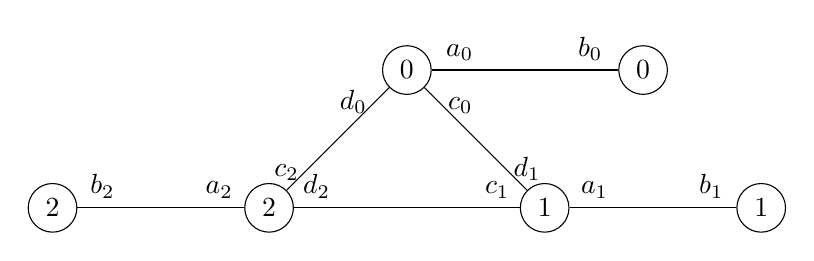
\begin{tikzpicture}
    \node[shape=circle,draw=black] (agent0) at ( 0.00, 0.00) {\tm{\agent0}};
    \node[shape=circle,draw=black] (agent1) at ( 1.75,-1.75) {\tm{\agent1}};
    \node[shape=circle,draw=black] (agent2) at (-1.75,-1.75) {\tm{\agent2}};
    \node[shape=circle,draw=black] (proc0)  at ( 3.00, 0.00) {\tm{\collector0}};
    \node[shape=circle,draw=black] (proc1)  at ( 4.50,-1.75) {\tm{\collector1}};
    \node[shape=circle,draw=black] (proc2)  at (-4.50,-1.75) {\tm{\collector2}};
    \node[draw=none]               (middle) at ( 0.00,-1.75) {};

    \draw
    (agent0) -- node[pos=0.35,above] {$c_0$}
    node[pos=1.0,above] {$d_1$} ++ (agent1);
    \draw
    (agent1) -- node[pos=0.1,above] {$c_1$}
    node[pos=0.9,above] {$d_2$} ++ (agent2);
    \draw
    (agent2) -- node[pos=0.0,above] {$c_2$}
    node[pos=0.65,above] {$d_0$} ++ (agent0);

    \draw
    (agent0) -- node[pos=0.15,above] {$a_0$}
    node[pos=0.85,above] {$b_0$} (proc0);
    \draw
    (agent1) -- node[pos=0.15,above] {$a_1$}
    node[pos=0.85,above] {$b_1$} (proc1);
    \draw
    (agent2) -- node[pos=0.15,above] {$a_2$}
    node[pos=0.85,above] {$b_2$} (proc2);
  \end{tikzpicture}
\end{center}
\[
  \begin{array}{lrlr}
    \tm{\sched}
    & \defeq & \tm{
               \res{a_0}{b_0}{\res{a_1}{b_1}{\res{a_2}{b_2}{
               \res{c_0}{d_1}{
               \res{c_1}{d_2}{
               \res{c_2}{d_0}{}}}}}}}
    \\ &     & \multicolumn{2}{l}{%
               \tm{(\ppar{\child\;\agent0}{\ppar{\child\;\agent1}{\child\;\ppar{\agent2}{
               \ppar{\child\;\collector0}{\ppar{\child\;\collector1}{\child\;\collector2}}}}})}}
    \\
    \tm{\agent0}
    & \defeq & \tm{\letbind{c_0}{\send\;\pair{\text{data}_0}{c_0}}{%
               \letpair{\text{data}'_0}{d_0}{\recv\;d_0}{}}}
    \\ &     & \tm{\letbind{a_0}{\send\;\pair{\text{data}_0}{a_0}}{}}
    \\ &     & \tm{\andthen{\wait\;{d_i}}{\andthen{\close\;{c_i}}{\close\;{a_i}}}}
    \\
    \tm{\agent{i}}
    & \defeq & \tm{\letpair{d_i}{d_i}{\recv\;d_i}{%
               \letbind{a_i}{\send\;\pair{\text{data}_i}{a_i}}{}}}
    \\ &     & \tm{\letpair{\text{data}'_i}{a_i}{\recv\;{a_i}}{%
               \letbind{c_i}{\send\;\pair{\text{data}_i}{c_i}}{}}}
    \\ &     & \tm{\andthen{\wait\;{d_i}}{\andthen{\close\;{c_i}}{\close\;{a_i}}}}
       & i \in \{1,2\}
    \\
    \tm{\collector{i}}
    & \defeq & \tm{\letpair{d'_i}{d_i}{\recv\;d_i}{M_i}}
       & i \in \{0,1,2\}
  \end{array}
\]

\subsection{Metatheory}

\begin{restatablelemma}{lempgvvaluedone}
  \label{lem:pgv-value-done}
  If $\tseq[\cs{p}]{\ty{\Gamma}}{V}{T}$, then $\cs{p}=\cs{\pbot}$, and $\minpr(\ty{\Gamma})=\minpr(\ty{T})$.
\end{restatablelemma}
\begin{proof}
  By induction on the derivation of $\tseq[\cs{p}]{\ty{\Gamma}}{V}{T}$.
  (Details in \cref{prf:lem-pgv-value-done}.)
\end{proof}

\begin{restatablelemma}{lempgvsubstitution}[Substitution]
  \label{lem:pgv-substitution}
  \hfill\\%newline before theorem statement
  If $\tseq[\cs{p}]{\ty{\Gamma},\tmty{x}{U'}}{M}{T}$ and $\tseq[\cs{q}]{\ty{\Theta}}{V}{U'}$, then $\tseq[\cs{p}]{\ty{\Gamma},\ty{\Theta}}{\subst{M}{V}{x}}{T}$.
\end{restatablelemma}
\begin{proof}
  By induction on the derivation of $\tseq[\cs{p}]{\ty{\Gamma},\tmty{x}{U'}}{M}{T}$. Whenever the contexts in the premises and conclusion differ, we use \cref{lem:pgv-value-done} to prove that the priorities are preserved.
  (Details in \cref{prf:lem-pgv-substitution}.)
\end{proof}

\begin{restatablelemma}{lempgvsubjectreductionterms}[Subject Reduction, $\tred$]
  \label{lem:pgv-subject-reduction-terms}
  \hfill\\%newline before theorem statement
  If $\tseq[\cs{p}]{\ty{\Gamma}}{M}{T}$ and $\tm{M}\tred\tm{M'}$,
  then $\tseq[\cs{p}]{\ty{\Gamma}}{M'}{T}$.
\end{restatablelemma}
\begin{proof}
  By induction on the derivation of $\tm{M}\tred\tm{M'}$.
  (Details in \cref{prf:lem-pgv-subject-reduction-terms}.)
\end{proof}

\begin{restatablelemma}{lempgvsubjectcongruence}[Subject Congruence, $\equiv$]
  \label{lem:pgv-subject-congruence}
  \hfill\\%newline before theorem statement
  If $\cseq[\phi]{\ty{\Gamma}}{\conf{C}}$ and $\tm{\conf{C}}\equiv\tm{\conf{C'}}$,
  then $\cseq[\phi]{\ty{\Gamma}}{\conf{C'}}$.
\end{restatablelemma}
\begin{proof}
  By induction on the derivation of $\tm{\conf{C}}\equiv\tm{\conf{C'}}$.
  (Details in \cref{prf:lem-pgv-subject-congruence}.)
\end{proof}

\begin{restatabletheorem}{thmpgvsubjectreductionconfs}[Subject Reduction, $\cred$]
  \label{thm:pgv-subject-reduction-confs}
  \hfill\\%newline before theorem statement
  If $\cseq[\phi]{\ty{\Gamma}}{\conf{C}}$ and $\tm{\conf{C}}\cred\tm{\conf{C'}}$,
  then $\cseq[\phi]{\ty{\Gamma}}{\conf{C'}}$.
\end{restatabletheorem}
\begin{proof}
  By induction on the derivation of $\tm{\conf{C}}\cred\tm{\conf{C'}}$.
  (Details in \cref{prf:thm-pgv-subject-reduction-confs}.)
\end{proof}

\begin{definition}[Actions]
  \label{def:pgv-actions}
  A~term acts on an endpoint $\tm{x}$ if it is of the form $\tm{\send\;\pair{V}{x}}$, $\tm{\recv\;{x}}$, $\tm{\close\;{x}}$, or $\tm{\wait\;{x}}$. A~term is an action if it acts on some endpoint $\tm{x}$.
\end{definition}

\begin{definition}[Ready Terms]
  \label{def:pgv-ready-actions}
  A~term $\tm{L}$ is ready if it is of the form $\tm{\plug{E}{M}}$, where $\tm{M}$ is of the form $\tm{\new}$, $\tm{\spawn\;N}$, $\tm{\link\;\pair{x}{y}}$ or $\tm{\link\;\pair{y}{x}}$, or $\tm{M}$ acts on $\tm{x}$. In the last case, we say that $\tm{L}$ is ready to act on $\tm{x}$.
\end{definition}

\begin{restatablelemma}{lempgvreadypriority}
  \label{lem:pgv-ready-priority}
  If $\tseq[\cs{p}]{\ty{\Gamma}}{L}{T}$ is ready to act on $\tmty{x}{S}\in\ty{\Gamma}$, then the priority bound $\cs{p}$ is some priority $\cs{o}$, \ie not $\cs{\pbot}$ or $\cs{\ptop}$.
\end{restatablelemma}
\begin{proof}
  Let $\tm{L}=\tm{\plug{E}{M}}$. By induction on the structure of $\tm{E}$. $\tm{M}$ has priority $\pr({\ty{S}})$, and each constructor of the evaluation context $\tm{E}$ passes on the \emph{maximum} of the priorities of its premises. No rule introduces the priority bound $\cs{\ptop}$ on the sequent.
\end{proof}

\begin{restatablelemma}{lempgvopenprogressterms}[Open Progress, $\tred$]
  \label{lem:pgv-open-progress-terms}
  If $\tseq[\cs{p}]{\ty{\Gamma}}{M}{T}$, then:
  \begin{itemize}
  \item $\tm{M}$ is a value;
  \item $\tm{M}\tred\tm{N}$ for some term $\tm{N}$; or
  \item $\tm{M}$ is ready.
  \end{itemize}
\end{restatablelemma}

\begin{definition}[Canonical Forms]
  \label{def:pgv-canonical-forms}
  A~configuration $\tm{\conf{C}}$ is in canonical form if it is of the following form, where no term $\tm{M_i}$ is a value:
  \[
    \tm{\res{x_1}{x'_1}{\dots\res{x_n}{x'_n}{(\child\;M_1\parallel\dots\parallel\child\;M_m\parallel\main\;N)}}}
  \]
\end{definition}

\begin{restatablelemma}{lempgvcanonicalforms}[Canonical Forms]
  \label{lem:pgv-canonical-forms}
  If $\cseq[\main]{\ty{\Gamma}}{\conf{C}}$, there exists some $\tm{\conf{D}}$ such that $\tm{\conf{C}}\equiv\tm{\conf{D}}$ and $\tm{\conf{D}}$ is in canonical form.
\end{restatablelemma}
\begin{proof}
  We move any $\nu$-binders to the top using \LabTirName{SC-ResExt}, discard any superfluous occurrences of $\tm{\child\;\unit}$ using \LabTirName{SC-ParNil}, and move the main thread to the rightmost position using \LabTirName{SC-ParComm} and \LabTirName{SC-ParAssoc}.
\end{proof}

\begin{restatabletheorem}{thmpgvclosedprogressconfs}[Closed Progress, $\cred$]
  \label{lem:pgv-closed-progress-confs}
  If $\cseq[\main]{\emptyenv}{\conf{C}}$ and $\tm{\conf{C}}$ is in canonical form, then either $\tm{\conf{C}}\cred\tm{\conf{D}}$ for some $\tm{\conf{D}}$; or
  \[
    \tm{\conf{C}}
    =
    \tm{\res{x_1}{x'_1}{\dots\res{x_n}{x'_n}{(\child\;M_1\parallel\dots\parallel\child\;M_m\parallel\main\;V)}}},
  \]
  where each $\tm{M_i}$ is ready to act on $\tm{x_i}$.
\end{restatabletheorem}
\begin{proof}
  Details in \cref{prf:thm-pgv-closed-progress-confs}.
\end{proof}

\end{document}

%%% Local Variables:
%%% TeX-master: "priorities"
%%% End:
